\section{Evaluation}%
\label{sec:eval}

\newsavebox{\IntelSizetIntReduced}
\begin{lrbox}{\IntelSizetIntReduced}
  \hspace{1.5em}
  \begin{lstlisting}
    kernel void A(global double* a) {
      int b = get_global_id(0);
      if (b < -1)
        a[b] = 1;
    }
  \end{lstlisting}
\end{lrbox}

\newsavebox{\OclgrindRaceSwitch}
\begin{lrbox}{\OclgrindRaceSwitch}
  \hspace{1.5em}
  \begin{lstlisting}
  kernel void A(global int* a, global int* b) {
    switch (get_global_id(0)) {
    case 0:
      a[get_global_id(0)]=b[get_global_id(0)+13];
      break;
    case 2:
      a[get_global_id(0)]=b[get_global_id(0)+11];
      break;
    case 6:
      a[get_global_id(0)]=b[get_global_id(0)+128];
    }
    barrier(2);
  }
  \end{lstlisting}
\end{lrbox}

\newsavebox{\AlmostEverythingCrash}
\begin{lrbox}{\AlmostEverythingCrash}
  \hspace{1.5em}
  \begin{lstlisting}
    kernel void A() {
      __builtin_astype(d, uint4);
    }
  \end{lstlisting}
\end{lrbox}

\newsavebox{\OclgrindSemaAssertion}
\begin{lrbox}{\OclgrindSemaAssertion}
  \hspace{1.5em}
  \begin{lstlisting}
    kernel void A(global unsigned char* a, global unsigned char* b) {
      unsigned long c = get_global_id(0);
      d[0] = (mad24(f, (int)(a[0], b[get_global_id(0)])) % (d * (d + 3)) + (c / 2))] * a[c + 1];
    }
  \end{lstlisting}
\end{lrbox}
% This has been forwarded to the LLVM folks https://bugs.llvm.org/show_bug.cgi?id=33897
% __kernel void A(__global float* b) {
%	(float4)(b);
% }

\newsavebox{\IntelPtrCompilerHang}
\begin{lrbox}{\IntelPtrCompilerHang}
  \hspace{1.5em}
  \begin{lstlisting}
    kernel void A(global ulong* a) {
      a[get_global_id(0)] = (ulong)(a + 1);
    }
  \end{lstlisting}
\end{lrbox}
% Another 3± hang:
% kernel void A(global const char* a, global char* b, global char* c) {
%   int d = get_global_id(0);
%   c[d] = get_global_id(0) + c;
% }

% Another 3± hang:
% __kernel void A(global int* a) {
%   local int b[4][3][4][5];
%   b[1][2][3][3] = b[3];
% }

\newsavebox{\NvidiaOptLoopHang}
\begin{lrbox}{\NvidiaOptLoopHang}
  \hspace{1.5em}
  % CLgenProgram.id = 6992
  \begin{lstlisting}
    kernel void A(global float* a, global float* b,
                  global float* c) {
      int d, e, f;
      d = get_local_id(0);
      for (int g = 0; g < 100000; g++)
        barrier(1);
    }
  \end{lstlisting}
\end{lrbox}

\newsavebox{\XeonPhiSpin}
\begin{lrbox}{\XeonPhiSpin}
  \hspace{1.5em}
  \begin{lstlisting}
    kernel void A(global unsigned char* a,
                  unsigned b) {
      a[get_global_id(0)] %= 42;
      barrier(1);
    }
  \end{lstlisting}
\end{lrbox}
% LLVM ERROR: LLVM2PIL: Cannot yet select: 0x7f72a45a7ed0: i8,i8 = umul_lohi 0x7f72a45a87d0, 0x7f72a45a88d0 [ORD=16] [ID=22]
% 0x7f72a45a87d0: i8 = srl 0x7f72a45a7dd0, 0x7f72a42fff90 [ORD=16] [ID=21]
% 0x7f72a45a7dd0: i8,ch = load 0x7f72a41d9438, 0x7f72a4300790, 0x7f72a4300590<LD1[%scevgep2]> [ORD=15] [ID=20]
% 0x7f72a4300790: i64 = add 0x7f72a45a83d0, 0x7f72a45a80d0 [ORD=14] [ID=17]
% 0x7f72a45a83d0: i64,ch = CopyFromReg 0x7f72a41d9438, 0x7f72a45a86d0 [ORD=14] [ID=13]
% 0x7f72a45a86d0: i64 = Register %vreg1 [ID=1]
% 0x7f72a45a80d0: i64,ch = CopyFromReg 0x7f72a41d9438, 0x7f72a45a81d0 [ORD=14] [ID=14]
% 0x7f72a45a81d0: i64 = Register %vreg2 [ID=2]
% 0x7f72a4300590: i64 = undef [ID=3]
% 0x7f72a42fff90: i8 = Constant<1> [ID=9]
% 0x7f72a45a88d0: i8 = Constant<49> [ID=10]

\newsavebox{\IntelOptLoopHang}
\begin{lrbox}{\IntelOptLoopHang}
  \hspace{1.5em}
  \begin{lstlisting}
    kernel void A(global int* a) {
      int b = get_global_id(0);
      while (b < 512) { }
    }
  \end{lstlisting}
\end{lrbox}
% Another example:
%   kernel void A(long a, long b) {
%     while (a > 273444) { }
%   }


\newsavebox{\NvidiaRecursionSegfault}
\begin{lrbox}{\NvidiaRecursionSegfault}
  \hspace{1.5em}
  \begin{lstlisting}
    kernel void A(float4 a, global float4* b, global float4* c, unsigned int d, global double* e, global int2* f, global int4* g, constant int* h, constant int* i) {
      A(a, b, c, d, d, e, f, g, h);
    }
  \end{lstlisting}
\end{lrbox}
% HAND REDUCED:
%
%   kernel void A(constant int2* a, global int* b) { A(b, a); }
\newsavebox{\NvidiaRecursionSegfaultReduced}
\begin{lrbox}{\NvidiaRecursionSegfaultReduced}
  \hspace{1.5em}
  \begin{lstlisting}
    kernel void B(constant int2* a, global int* b) {
      A(b, a);
    }
  \end{lstlisting}
\end{lrbox}

\newsavebox{\BeignetScalarizeInsert}
\begin{lrbox}{\BeignetScalarizeInsert}
  \hspace{1.5em}
  \begin{lstlisting}
    kernel void A(global float4* a) {
      a[get_local_id(0) / 8][get_local_id(0)] = get_local_id(0);
    }
  \end{lstlisting}
\end{lrbox}

\newsavebox{\OclgrindUncorrectedTypos}
\begin{lrbox}{\OclgrindUncorrectedTypos}
  \hspace{1.5em}
  \begin{lstlisting}
    kernel void A(global float* a, global float* b) {
      a[0] = max(a[c], b[2]);
    }
  \end{lstlisting}
\end{lrbox}

\newsavebox{\BeignetPtrIntSpin}
\begin{lrbox}{\BeignetPtrIntSpin}
  \hspace{1.5em}
  \begin{lstlisting}
    kernel void A(global int* a) {
      int b = get_global_id(0);
      a[b] = (6 * 32) + 4 * (32 / 32) + a;
    }
  \end{lstlisting}
\end{lrbox}

\newsavebox{\NvidiaCompileSegfault}
\begin{lrbox}{\NvidiaCompileSegfault}
  \hspace{1.5em}
  \begin{lstlisting}
    kernel void A(global float* a, local float* b, local float* c, int d, int e) {
      int f, g;
      int h = get_local_id(0);
      int i = get_local_id(1);
      int j = get_global_id(0);
      global char* k = c + f * g + f;
      if (f + 1 < h)
        b[f * d + g * h + g] = g * f;
    }
  \end{lstlisting}
\end{lrbox}

\newsavebox{\XeonPhiSegfault}
\begin{lrbox}{\XeonPhiSegfault}
  \hspace{1.5em}
  \begin{lstlisting}
    kernel void A(void) {
      global int* a;
      unsigned int* b;
      b = a[0];
      a[0] = b;
      a[0] = b;
      barrier(1);
      if (get_global_id(0) == 0)
        *a = 0;
      a[get_local_id(0)] = 0;
    }
  \end{lstlisting}
\end{lrbox}

\newsavebox{\IntelVectorizerSegfault}
\begin{lrbox}{\IntelVectorizerSegfault}
  \hspace{1.5em}
  \begin{lstlisting}
    kernel void A() {
      while (true) {
        barrier(1);
      }
    }
  \end{lstlisting}
\end{lrbox}

\newsavebox{\IntelSizetIntUnreduced}
\begin{lrbox}{\IntelSizetIntUnreduced}
  \hspace{1.5em}
  \begin{lstlisting}
    kernel void A(global double* a, global double* b,
                  global double* c, int d, int e) {
      double f;
      int g = get_global_id(0);
      if (g < e - d - 1)
        c[g] = (((e) / d) % 5) % (e + d);
    }
  \end{lstlisting}
\end{lrbox}

\newsavebox{\PoclUndefinedSymbols}
\begin{lrbox}{\PoclUndefinedSymbols}
  \hspace{1.5em}
  \begin{lstlisting}
    kernel void A(local int* a) {
      for (int b = 0; b < 100; b++)
        B(a);
    }
  \end{lstlisting}
\end{lrbox}


\newsavebox{\BeignetCastError}
\begin{lrbox}{\BeignetCastError}
  \hspace{1.5em}
  \begin{lstlisting}
    kernel void A(global float* a, global float* b, global float* c, const int d) {
      int e = get_global_id(0);
      if (e < d)
        c[e] = a[e] + b[e];
      b[e] = (char)(c[e] + d);
    }
  \end{lstlisting}
\end{lrbox}

\newsavebox{\XeonPhiInvalidWrite}
\begin{lrbox}{\XeonPhiInvalidWrite}
  \hspace{1.5em}
  \begin{lstlisting}
    kernel void A(global int* a) {
      a[0] = 1;
      a[-1] = 2;
      a[0] = 3;
    }
  \end{lstlisting}\cc{TODO:}
\end{lrbox}

\newsavebox{\UninitRead}
\begin{lrbox}{\UninitRead}
  \hspace{1.5em}
  \begin{lstlisting}
      kernel void A(global int* a, global int* b) {
        int c[16];
        int d = get_global_id(0);
        a[d] = b[d] + c[d];
      }
  \end{lstlisting}
\end{lrbox}

\newsavebox{\IntelPtrAssertion}
\begin{lrbox}{\IntelPtrAssertion}
  \hspace{1.5em}
  \begin{lstlisting}
    kernel void A(global int* a, global int* b) {
      int c = (int)get_global_id(0);
      a[c] += b;
    }
  \end{lstlisting}
\end{lrbox}

\newsavebox{\IntelScalarAssertion}
\begin{lrbox}{\IntelScalarAssertion}
  \hspace{1.5em}
  \begin{lstlisting}
    kernel void A(global float* a, global float* b, global float* c, local float* d, unsigned int e, unsigned int f) {
      for (unsigned int g = get_local_id(0) + get_local_size(0); g < get_local_size(0); g += get_local_size(0))
        a[2 * get_local_id(0) + 1] = get_local_id(0);
    }
  \end{lstlisting}
\end{lrbox}

\newsavebox{\BeignetTernary}
\begin{lrbox}{\BeignetTernary}
  \hspace{1.5em}
  \begin{lstlisting}
    kernel void A(global int* a, global int* b, 
                  global int* c) {
      c[0] = (a[0] > b[0]) ? a[0] : 0;
      c[2] = (a[3] <= b[3]) ? a[4] : b[5];
      c[4] = (a[4] <= b[5]) ? a[7] : b[7];
      c[7] = (a[7] < b[0]) ? a[0] : (a[0] > b[1]);
    }
  \end{lstlisting}
\end{lrbox}
% HAND REDUCED:
%
%   kernel void A(global int* a, global int* b, global int* c) {
%     c[0] = 100;
%     c[1] = (a[3] <= b[4]) ? a[4] : b[5];
%   }

\newsavebox{\BeignetTernarySmaller}
\begin{lrbox}{\BeignetTernarySmaller}
  \hspace{1.5em}
  \begin{lstlisting}
    kernel void A(global int* a, global int* b, global int* c) {
      c[0] = (a[0] > 0) ? a[0] : b[1];
      c[1] = (a[1] <= b[1]) ? a[0] : b[0];
    }
  \end{lstlisting}
\end{lrbox}

\newsavebox{\IntelGtDoubleAssertion}
\begin{lrbox}{\IntelGtDoubleAssertion}
  \hspace{1.5em}
  \begin{lstlisting}
    kernel void A(read_only image2d_t a, global double2* b) {
      b[0] = get_global_id(0);
    }
  \end{lstlisting}
\end{lrbox}

\newsavebox{\IntelDeclDoesntDeclareAnything}
\begin{lrbox}{\IntelDeclDoesntDeclareAnything}
  \hspace{1.5em}
  \begin{lstlisting}
    kernel void A() {
      char a;
      int b;
      int const;
    }
  \end{lstlisting}
\end{lrbox}

\newsavebox{\AddressQualifiedAutoVar}
\begin{lrbox}{\AddressQualifiedAutoVar}
  \hspace{1.5em}
  \begin{lstlisting}
    kernel void A(global float4* a, global float4* b, global float4* c, global float4* d, global float4* e, float f) {
      unsigned int g = get_global_id(0);
      int h = get_global_size(0);
      constant sampler_t i = 0x0000 | 0x0004 | 0x0000;
      unsigned int j = g * (1 << ((h % 4) - (2)));
    }
  \end{lstlisting}
\end{lrbox}

\newsavebox{\NvidiaLocalGlobalSegfault}
\begin{lrbox}{\NvidiaLocalGlobalSegfault}
  \hspace{1.5em}
  \begin{lstlisting}
    kernel void A(global int* a) {
      local int b[2][3][4][5];
      if (get_global_id(0) == 0)
        a = b[0];
    }
  \end{lstlisting}
\end{lrbox}

\newsavebox{\NvidiaLocalSegfault}
\begin{lrbox}{\NvidiaLocalSegfault}
  \hspace{1.5em}
  \begin{lstlisting}
    kernel void A(global uchar4* a, const int b) {
      local int c[16];
      local float8* d = a + 133;
      atomic_cmpxchg(c, 10, 13);
    }
  \end{lstlisting}
\end{lrbox}


% Program ID: 35612
\newsavebox{\IntelPostDominanceFrontier}
\begin{lrbox}{\IntelPostDominanceFrontier}
  \hspace{1.5em}
  \begin{lstlisting}
    kernel void A() {
      while (true)
        barrier(1);
    }
  \end{lstlisting}
\end{lrbox}
% Another:
% kernel void A(local int* a) {
%   while (1) {
%   }
% }
%
% And another:
%    kernel void A(global int* a) {
%      bool b;
%      int c;
%      for (b = 0; b < 100; b++)
%        a[c] += a[c];
%    }
%
% One more:
%   kernel void A(global int* a, global int* b) {
%     int c = get_global_id(0);
%     int d = 0;
%     while (d < 1024)
%       a[c] = d;
%   }

\newsavebox{\IntelPredicator}
\begin{lrbox}{\IntelPredicator}
  \hspace{1.5em}
  \begin{lstlisting}
    kernel void A(global int* a) {
      int b = get_global_id(0);
      while (b < *a)
        if (a[0] < 0)
          a[1] = b / b * get_local_id(0);
    }
  \end{lstlisting}
\end{lrbox}

\newsavebox{\IntelPrepareKernelArgs}
\begin{lrbox}{\IntelPrepareKernelArgs}
  \hspace{1.5em}
  \begin{lstlisting}
    kernel void A(int a, global int* b) {
      int c = get_global_id(0);
      int d = work_group_scan_inclusive_max(c);
      b[c] = c;
    }
  \end{lstlisting}
\end{lrbox}

\newsavebox{\IntelDAGInstrSelection}
\begin{lrbox}{\IntelDAGInstrSelection}
  \hspace{1.5em}
  \begin{lstlisting}
    kernel void A(global half* a, global int* b, global bool* c, int d, int e) {
      int f = get_global_id(0);
      int g = get_global_id(1) * e;
      if (f < e)
        a[f] = b[f];
    }
  \end{lstlisting}
\end{lrbox}

\newsavebox{\IntelSPIRMetadata}
\begin{lrbox}{\IntelSPIRMetadata}
  \hspace{1.5em}
  \begin{lstlisting}
    kernel void A() {
      local float a;
      A(a);
    }
  \end{lstlisting}
\end{lrbox}

\newsavebox{\IntelRemoveDupeBarrier}
\begin{lrbox}{\IntelRemoveDupeBarrier}
  \hspace{1.5em}
  \begin{lstlisting}
    kernel void A() {
      local int a[10];
      local int b[16][16];
      a[1024 + (2 * get_local_id(1) +
        get_local_id(0)) + get_local_id(0)] = 6;
      barrier(b);
    }
  \end{lstlisting}
\end{lrbox}

\newsavebox{\IntelCombineRedundant}
\begin{lrbox}{\IntelCombineRedundant}
  \hspace{1.5em}
  \begin{lstlisting}
    kernel void A(global float* a, global float* b,
                  global float* c, const int d) {
      for (unsigned int e = get_global_id(0);
           e < d; e += get_global_size(0))
        for (unsigned f = 0; f < d; ++f)
          e += a[f];
    }
  \end{lstlisting}
\end{lrbox}


\newsavebox{\BeigPtrAssertion}
\begin{lrbox}{\BeigPtrAssertion}
  \hspace{1.5em}
  \begin{lstlisting}
    kernel void A(global int* a, global int* b,
                  global int* c) {
      a[get_global_id(0)] = a[get_global_id(0)] > b;
    }
  \end{lstlisting}
\end{lrbox}

\newsavebox{\BeigIterAssertion}
\begin{lrbox}{\BeigIterAssertion}
  \hspace{1.5em}
  \begin{lstlisting}
    kernel void A(global int* a) {
      global int* b = ((void*)0);
      b[0] = a;
    }
  \end{lstlisting}
\end{lrbox}

\newsavebox{\ParserFailOne}
\begin{lrbox}{\ParserFailOne}
  \hspace{1.5em}
  \begin{lstlisting}
    void A(){(global a*)()
  \end{lstlisting}
\end{lrbox}

\newsavebox{\ParserFailTwo}
\begin{lrbox}{\ParserFailTwo}
  \hspace{1.5em}
  \begin{lstlisting}
    void A(){void* a; uint4 b=0; b=(b>b)?a:a
  \end{lstlisting}
\end{lrbox}

\newsavebox{\ParserFailThree}
\begin{lrbox}{\ParserFailThree}
  \hspace{1.5em}
  \begin{lstlisting}
    void A(){double2 k; return (float4)(k, k, k, k)
  \end{lstlisting}
\end{lrbox}

\noindent
We report on the results of DeepSmith testing of the 10 OpenCL systems from Table~\ref{tab:platforms}, in which each ran for 48 hours.
% \cc{TODO: Address the concern that generating samples from codebases of working programs may not trigger bugs that are linked to unusual programming styles.}
We found bugs in all the compilers we tested --- every compiler crashed, and every compiler generated programs which either crash or silently compute the wrong result. To date, we have submitted \factcheck{67} bug reports to compiler vendors. We first provide a qualitative analysis of compile-time and runtime defects found, followed by a quantitative comparison of our approach against the state-of-the-art in OpenCL compiler fuzzing --- CLSmith~\cite{Lidbury2015a}. DeepSmith is able to identify a broad range of defects, many of which CLSmith cannot, for only a fraction of the engineering effort. Finally, we provide a quantitative analysis of compiler robustness over time, using the compiler crash rate of every LLVM release in the past two years as a metric of compiler robustness. We find that progress is good, compilers are becoming more robust, yet the introduction of new features and regressions ensures that compiler validation remains a moving target.

%Unless stated otherwise, all code listings are presented verbatim as generated by DeepSmith --- only uneeded whitespace and braces have been removed to save space.

Unless stated otherwise, DeepSmith code listings are presented verbatim, with only minor formatting changes applied to save space. No test case reduction, either manual or automatic, was needed.

% We use a shorthand to refer to specific testbed configurations. $1+$ means Testbed 1 with optimizations enabled, $2-$ means Testbed 2 with optimizations disabled, and $3\pm$ means Testbed 3 with either optimizations enabled or disabled.

For the remainder of the paper we identify testbeds using the OpenCL system number from Table~\ref{tab:platforms}, suffixed with $+$, $-$, or $\pm$ to denote optimizations on, off, or either, respectively.

\subsection{Compile-time Defects}%
\label{subsec:compile-time-defects}

OpenCL is typically compiled online, which amplifies the significance of detecting compile-time defects, as they may not be discovered until code has been shipped to customers. We found numerous cases where DeepSmith kernels trigger a crash in the compiler (and as a result, the host process), or cause the compiler to loop indefinitely. In the testing time allotted we have identified 199 test cases which trigger unreachable code failures, triggered 31 different compiler assertions, and produced 114 distinct stack traces from other compiler crashes.

\begin{figure}
  \centering %
  \subfloat[Testbeds $10\pm$ assertion \emph{Uncorrected typos!} during semantic analysis.]{%
    \noindent\mbox{\parbox{\columnwidth}{\usebox{\OclgrindUncorrectedTypos}}}%
    \label{lst:oclgrind-uncorrected-typos}
  }\\%
  \subfloat[Testbeds $1\pm$, $2\pm$ segmentation fault due to implicit address space conversion.]{%
    \noindent\mbox{\parbox{\columnwidth}{\usebox{\NvidiaRecursionSegfault}}}%
    \label{lst:nvidia-recursion-segfault}
  }\\%
  \subfloat[Testbeds $3\pm$ assertion \emph{sel.hasDoubleType()} during code generation.]{%
    \noindent\mbox{\parbox{\columnwidth}{\usebox{\IntelGtDoubleAssertion}}}%
    \label{lst:intel-gt2-double-assertion}
  }\\%
  \subfloat[Testbeds $3\pm$ assertion \emph{scalarizeInsert} during code generation.]{%
    \noindent\mbox{\parbox{\columnwidth}{\usebox{\BeignetScalarizeInsert}}}%
    \label{lst:beignet-scalarize-insert}
  }\\%
  \subfloat[Of the 10 compilers we tested, 6 crash with segfault when compiling this kernel.%
    % \cc{TODO: Which six?}
    ]{%
    \noindent\mbox{\parbox{\columnwidth}{\usebox{\AlmostEverythingCrash}}}%
    \label{lst:almost-everything-crash}
  }\\%
  \caption{Example kernels which crash compilers.}%
\end{figure}

\begin{figure}
	\centering %
	\subfloat[Reduced from 48 line kernel.]{%
		\noindent\mbox{\parbox{\columnwidth}{\usebox{\ParserFailOne}}}%
	}\\%
	\subfloat[Reduced from 52 line kernel.]{%
		\noindent\mbox{\parbox{\columnwidth}{\usebox{\ParserFailTwo}}}%
	}\\%
	\subfloat[Reduced from 68 line kernel.]{%
		\noindent\mbox{\parbox{\columnwidth}{\usebox{\ParserFailThree}}}%
	}\\%
	\caption{Example codes which crash parsers.}%
	\label{lst:parser-crashes}%
\end{figure}

\paragraph{Semantic Analysis Failures} %
Compilers should produce meaningful diagnostics when inputs are invalid, yet we discovered dozens of compiler defects attributable to improper or missing error handling. Many generation and mutation based approaches to on compiler validation have focused solely on testing under \emph{valid inputs}. As such, this class of bugs may go undiscovered. We believe that our approach contributes a significant improvement to generating plausibly-erroneous code over prior random-enumeration approaches.

The use of undeclared identifiers is a core error diagnostic which one would expect to be robust in a mature compiler. DeepSmith discovered cases in which the presence of undeclared identifiers causes the Testbeds $10\pm$ compiler to crash. For example, the undeclared identifier \texttt{c} in Figure~\ref{lst:oclgrind-uncorrected-typos} raises an assertion during semantic analysis of the AST when used as an array index.

Type errors were an occasional cause of compile-time defect. Figure~\ref{lst:nvidia-recursion-segfault} induces a crash in NVIDIA compilers due to an implicit conversion between global to constant address qualifiers. Worse, we found that Testbeds $3\pm$ would loop indefinitely on some kernels containing implicit conversions from a pointer to an integer, as shown in Figure~\ref{lst:beignet-ptr-int-spin}. While spinning, the compiler would utilize 100\% of the CPU and consume an increasing amount of host memory until the entire system memory is depleted and the process crashes. % This would be a nice one to have fixed.

% \paragraph{Code Generation} %
Occasionally, incorrect program semantics will remain undetected until late in the compilation process. Both Figures~\ref{lst:intel-gt2-double-assertion} and~\ref{lst:beignet-scalarize-insert} pass the type checker and semantic analysis, but trigger compiler assertions during code generation.

% \paragraph{Compiler-specific Code} %
An interesting yet unintended byproduct of having trained DeepSmith on thousands of real world examples is that the model learned to occasionally generate compiler-specific code, such as invoking compiler builtins. We found the quality of error handling on these builtins to vary wildly. For example, Figure~\ref{lst:almost-everything-crash} silently crashes 6 of the 10 compilers, which, to the best of our knowledge, makes DeepSmith the first random program generator to induce a defect through exploiting compiler-specific functionality.

% Since the expressiveness of our approach is bounded only by the handwritten programs we train on, DeepSmith will occasionally emit compiler-specific code

% CLgen result ID 994
% TODO: Testbed $3\pm$ assertion in \emph{gbe::GenEncoder::handleDouble}

\paragraph{Parser Failures} %
Parser development is a mature and well understood practice. We uncovered parser errors in several compilers. Each of the code samples in Figure~\ref{lst:parser-crashes} induce crash errors during parsing of compound statements in both Testbeds $5\pm$ and $7\pm$. For space, we have hand-reduced the listings to minimal code samples, which we have reported to Intel. Each reduction took around 6 edit-compile steps, taking less than 10 minutes. In total, we have generated 100 distinct programs which crash compilers during parsing.

\begin{figure}
  \centering %
  \subfloat[Testbeds $3\pm$ loop indefinitely, leaking memory until the entire system memory is depleted and the process crashes.]{%
    \noindent\mbox{\parbox{\columnwidth}{\usebox{\BeignetPtrIntSpin}}}%
    \label{lst:beignet-ptr-int-spin}
  }\\%
  \subfloat[Testbed $1+$ hangs during optimization of kernels with large loop bounds. Testbeds $1-$ and $2\pm$ compile in under 1 second.]{%
    \noindent\mbox{\parbox{\columnwidth}{\usebox{\NvidiaOptLoopHang}}}%
    \label{lst:nvidia-opt-loop-hang}
  }\\%
  \subfloat[Testbeds $4+$, $5+$, $6+$, $7+$ hang during optimization of kernels with non-terminating loops.]{%
    \noindent\mbox{\parbox{\columnwidth}{\usebox{\IntelOptLoopHang}}}%
    \label{lst:intel-inf-loop}
  }\\%
  \subfloat[Testbeds $7\pm$ loops indefinitely, consuming 100\% CPU usage.]{%
    \noindent\mbox{\parbox{\columnwidth}{\usebox{\XeonPhiSpin}}}%
    \label{lst:xeon-phi-spin}
  }\\%
  \caption{Example kernels which hang compilers.}%
  \label{lst:compiler-hangs}%
\end{figure}

\paragraph{Compiler Hangs} %
As expected, some compile-time defects are optimization sensitive. Testbed $1+$ \factcheck{hangs on large loop bounds}, shown in Figure~\ref{lst:nvidia-opt-loop-hang}. All commercial Intel compilers we tested \factcheck{hang during optimization of non-terminating loops} (Figure~\ref{lst:intel-inf-loop}).

Testbeds $7\pm$ \factcheck{loop indefinitely during compilation of the simple kernel} in Figure~\ref{lst:xeon-phi-spin}.

\paragraph{Other errors} %

Some compilers are more permissive than others. Testbeds~$4\pm$, $6\pm$, $9\pm$ reject out-of-range literal values e.g. \texttt{int i = 0xFFFFFFFFFFFFFFFFFFFFFFFF}, whilst Testbeds $3\pm$, $5\pm$, $7\pm$, $8\pm$, and $10\pm$ interpret the literal as an \texttt{unsigned long long} and implicitly cast to an integer value of \texttt{-1}. Testbeds $1\pm$, $2\pm$ emit no warning.

\factcheck{Testbeds~$1\pm$, $2\pm$, $3\pm$ rejected address space qualifiers on automatic variables}, where all other testbeds successfully compiled and executed.

On Testbeds~$3\pm$, the statement \texttt{int n = mad24(a, (32), get\_global\_size(0));} (a call to a math builtin with mixed types) \factcheck{is rejected as ambiguous}.

% 110 distinct test cases which crash testbed $9\pm$ during compilation, all silently.

% \begin{figure}
%   \centering %
%   \subfloat[]{%
%     \noindent\mbox{\parbox{\columnwidth}{\usebox{\NvidiaLocalGlobalSegfault}}}%
%     \label{lst:nvidia-local-global-sefault}
%   }\\%
%   \subfloat[]{%
%       \noindent\mbox{\parbox{\columnwidth}{\usebox{\NvidiaLocalSegfault}}}%
%       \label{lst:nvidia-local-global-sefault}
%     }\\%
%   \caption{Kernels containing pointer assignments which segfault Nvidia compilers.}%
%   \label{lst:nvidia-silent-segfaults}
% \end{figure}
%
% This makes identifying root causes more difficult. Figure~\ref{lst:nvidia-silent-segfaults} shows examples of crashes we identified as caused by pointer assignments. Without error messages and access to the compiler source code, we can only report a couple of errors and move on.
%


%\begin{figure}
%  \centering %
%  \subfloat[Testbeds $1\pm$, $2\pm$, $3\pm$ reject address space-qualified automatic variables.]{%
%    \noindent\mbox{\parbox{\columnwidth}{\usebox{\AddressQualifiedAutoVar}}}%
%    \label{lst:adress-qualified-autovar}
%  }\\%
%  \subfloat[Testbeds $4\pm$, $6\pm$ reject anonymous declarations. %\emph{declaration doesn't declare anything}.
%    % All other testbeds compile, some with a warning.
%    ]{%
%    \noindent\mbox{\parbox{\columnwidth}{\usebox{\IntelDeclDoesntDeclareAnything}}}%
%    \label{lst:intel-decl-doesnt-declare-anything}
%  }\\%
%  \caption{Well-formed kernels which do not compile.}%
%\end{figure}


\subsection{Runtime Defects}
\label{subsec:runtime-defects}

\begin{figure}
  \centering %
  \subfloat[Testbeds $4+$, $6+$ incorrectly optimize the \texttt{if} statement, causing the conditional branch to execute (it shouldn't). This pattern of integer comparison to thread ID is widely used.]{%
    \noindent\mbox{\parbox{\columnwidth}{\usebox{\IntelSizetIntUnreduced}}}%
    \label{lst:intel-size_t-int-unreduced}
  }\\%
  \subfloat[A race condition in \texttt{switch} statement evaluation causes $10\pm$ to sporadically crash when executed with a number of threads $> 1$.]{%
    \noindent\mbox{\parbox{\columnwidth}{\usebox{\OclgrindRaceSwitch}}}%
    \label{lst:oclgrind-race-switch}
  }\\%
  \subfloat[Testbeds $3\pm$ silently miscompile ternary assignments in which the operands are different global buffers.]{%
    \noindent\mbox{\parbox{\columnwidth}{\usebox{\BeignetTernary}}}%
    \label{lst:beig-ternary-ops}
  }\\%
  \subfloat[Compilation should fail due to call to undefined function \texttt{B()}; Testbeds $8\pm$ silently succeed then crash upon kernel execution.]{%
    \noindent\mbox{\parbox{\columnwidth}{\usebox{\PoclUndefinedSymbols}}}%
    \label{lst:pocl-undefined-symbols}
  }\\%
%  \subfloat[Testbeds $3\pm$ incorrect cast yields \texttt{b[e] = 127}, not \texttt{b[e] = 0}. \cc{TODO: Is char overflow defined?}]{%
%    \noindent\mbox{\parbox{\columnwidth}{\usebox{\BeignetCastError}}}%
%    \label{lst:beignet-cast-error}
%  }\\%
  \caption{Example kernels which are miscompiled.}%
\end{figure}

Prior work on compiler test case generation has focused on extensive stress-testing of compiler middle-ends to uncover miscompilations~\cite{Chen2014a}. CSmith, and by extension, CLSmith, specifically targets this class of bugs. Grammar based enumeration is highly effective at this task, yet is bounded by the expressiveness of the grammar. Here we provide examples of bugs which cannot currently be discovered by CLSmith.

\paragraph{Thread-dependent Flow Control} A common pattern in OpenCL is to obtain the thread identity, often as an \texttt{int}, and to compare this against some fixed value to determine whether or not to complete a unit of work (\factcheck{46\% of OpenCL kernels on GitHub use this ($tid \rightarrow$ int, \texttt{if (tid < \ldots) \{\ldots\}}) pattern}). DeepSmith, having modeled the frequency with which this pattern occurs in real handwritten code, generates many permutations of this pattern. And in doing so, exposed a bug in the optimizer of Testbeds $4+$ and $6+$ which causes the \texttt{if} branch in Figure~\ref{lst:intel-size_t-int-unreduced} to be erroneously executed when the kernel is compiled with optimizations enabled. We have reported this issue to Intel. CLSmith does not permit the thread identity to modify control flow, rendering such productions impossible.

Figure~\ref{lst:oclgrind-race-switch} shows a simple program in which thread identity determines the program output. We found that this test case would sporadically crash Testbeds~$10\pm$, an OpenCL device simulator and debugger. Upon reporting to the developers, the underlying cause was quickly diagnosed as a race condition in \texttt{switch} statement evaluation, and fixed within a week.

\paragraph{Kernel Inputs} CLSmith kernels accept a single buffer parameter into which each thread computes its result. This fixed prototype limits the ability to detect bugs which depend on input arguments. Figure~\ref{lst:beig-ternary-ops} exposes a bug of this type. Testbeds $3\pm$ \factcheck{will silently miscompile ternary operators when the ternary operands consist of values stored in multiple different global buffers}. CLSmith, with its fixed single input prototype, is unable to discover this bug. % All data is allocated statically in global structs.

\paragraph{Latent Compile-time Defects} Sometimes, invalid compiler inputs may go undetected, leading to runtime defects only upon program execution. Since CLSmith enumerates only well-formed programs, this class of bugs cannot be discovered.

Figure~\ref{lst:pocl-undefined-symbols} exposes a bug in which a kernel containing an \factcheck{undefined symbol} will successfully compile without warning on Testbeds~$8\pm$, then crash the program when attempting to run the kernel. This issue has been reported to the developers and fixed.

%\subsection{Gray Areas and False Positives}
%
%None of the three statements in Figure~\ref{lst:xeon-phi-invalid-write} are executed by testbeds~$7\pm$, all other configurations return the final value. In testbeds $1\pm$ (but not $2\pm$), out-of-bounds memory reads and writes can be used to overflow into neighboring kernel arguments. In both cases, oclgrind can automatically catch the inalid accesses to prevent false-positives, but perhaps should results may be interesting for testing robustness / security. E.g.~\cite{Holler2012}.
%
%
%
%\begin{figure}
%  \centering %
%  \subfloat[The out-of-range write on line 3 is invalid, but does not affect execution of lines 2 and 4 for all testbeds except $7\pm$. On Testbeds $7\pm$, lines 2 and 4 execute when the invalid write has an index $1 \le i < 44032$, and not  when index $i \ge 44032$ or $i < 0$.]{%
%    \noindent\mbox{\parbox{\columnwidth}{\usebox{\XeonPhiInvalidWrite}}}%
%    \label{lst:xeon-phi-invalid-write}
%  }\\%
%  \caption{Example kernels which mis-match.}%
%  \label{lst:gray-areas}%
%\end{figure}
%
%\begin{figure}
%  \centering %
%  \subfloat[Read of uninitialized automatic variable \texttt{c}.]{%
%    \noindent\mbox{\parbox{\columnwidth}{\usebox{\UninitRead}}}%
%    \label{lst:uninit-read}
%  }\\%
%  \caption{False positives.}%
%  \label{lst:uninit-read}%
%\end{figure}


\subsection{Comparison to State-of-the-art}%
\label{subsec:vs_clsmith}

In this section, we provide a quantitative comparison of the bug-finding capabilities of DeepSmith and CLSmith.

\paragraph{Results Overview}

\begin{table*}
  \scriptsize %
  \centering %
  \begin{tabular}{lll | rrrrr | rrrrr }
  \toprule
  & & & \multicolumn{5}{c|}{\textbf{CLSmith}} & \multicolumn{5}{c}{\textbf{CLgen}} \\
  \textbf{\#.} & \textbf{Device} & $\pm$ &
  \textbf{w} & \textbf{bf} & \textbf{c} & \textbf{to} & \textbf{\% of total} &
  \textbf{w} & \textbf{bf} & \textbf{c} & \textbf{to} & \textbf{\% of total} \\
  \midrule
  \multirow{ 2}{*}{1} & \multirow{ 2}{*}{GeForce GTX 1080} & $-$ & 0 & 0 & 17 & 25 & 0.8\%       & 10 & 45 & 28 & 5 & 0.4\% \\& & $+$ & 5 & 0 & 63 & 15 & 1.5\% & 14 & 28 & 12 & 14 & 0.3\% \\
\hline
\multirow{ 2}{*}{2} & \multirow{ 2}{*}{GeForce GTX 780} & $-$ & 3 & 0 & 22 & 37 & 0.9\%       & 617 & 406 & 65 & 42 & 25.9\% \\& & $+$ & 0 & 0 & 10 & 37 & 0.7\% & 281 & 375 & 37 & 68 & 22.9\% \\
\hline
\multirow{ 2}{*}{3} & \multirow{ 2}{*}{Intel HD Haswell GT2} & $-$ & 0 & 0 & 0 & 0 & 0.0\%       & 108 & 473 & 20 & 0 & 1.2\% \\& & $+$ & 0 & 0 & 0 & 0 & 0.0\% & 22 & 39 & 6 & 0 & 0.2\% \\
\hline
\multirow{ 2}{*}{4} & \multirow{ 2}{*}{Intel E5-2620 v4} & $-$ & 0 & 563 & 192 & 0 & 11.2\%       & 3 & 10 & 93 & 1 & 0.3\% \\& & $+$ & 0 & 595 & 434 & 1 & 14.5\% & 1 & 7 & 110 & 3 & 0.3\% \\
\hline
\multirow{ 2}{*}{5} & \multirow{ 2}{*}{Intel E5-2650 v2} & $-$ & 0 & 0 & 0 & 0 & 0.0\%       & 2 & 65 & 131 & 1 & 23.9\% \\& & $+$ & 0 & 0 & 61 & 0 & 1.1\% & 8 & 66 & 138 & 3 & 25.1\% \\
\hline
\multirow{ 2}{*}{6} & \multirow{ 2}{*}{Intel i5-4570} & $-$ & 0 & 570 & 0 & 0 & 8.3\%       & 15 & 362 & 156 & 10 & 20.2\% \\& & $+$ & 0 & 629 & 0 & 0 & 8.2\% & 6 & 167 & 170 & 10 & 31.6\% \\
\hline
\multirow{ 2}{*}{7} & \multirow{ 2}{*}{Intel Xeon Phi} & $-$ & 6 & 0 & 131 & 5 & 2.8\%       & 19 & 30 & 0 & 73 & 0.9\% \\& & $+$ & 1 & 0 & 0 & 4 & 0.3\% & 12 & 32 & 0 & 65 & 0.8\% \\
\hline
\multirow{ 2}{*}{8} & \multirow{ 2}{*}{POCL (Intel E5-2620)} & $-$ & 0 & 0 & 56 & 2 & 0.9\%       & 2 & 6 & 850 & 7 & 2.8\% \\& & $+$ & 0 & 0 & 8 & 18 & 0.4\% & 1 & 7 & 930 & 1 & 2.9\% \\
\hline
\multirow{ 2}{*}{9} & \multirow{ 2}{*}{ComputeAorta (Intel E5-2620)} & $-$ & 0 & 0 & 0 & 11 & 0.2\%       & 15 & 620 & 85 & 0 & 38.8\% \\& & $+$ & 9 & 0 & 177 & 35 & 3.1\% & 19 & 563 & 49 & 6 & 39.4\% \\
\hline
\multirow{ 2}{*}{10} & \multirow{ 2}{*}{Oclgrind Simulator} & $-$ & 0 & 0 & 0 & 8 & 0.4\%       & 6 & 3 & 13 & 80 & 0.3\% \\& & $+$ & 0 & 0 & 0 & 14 & 0.7\% & 7 & 2 & 9 & 50 & 0.2\% \\
  \bottomrule
\end{tabular}


  \caption{%
    % CLSmith total ``interesting'': 19415
    % DeepSmith total ``interesting'': 8272
    Results from 48 hours of testing using CLSmith and DeepSmith. System \#. as per Table~\ref{tab:platforms}. $\pm$ denotes optimizations off ($-$) vs on ($+$). The remaining columns denote the number of build crash (\bc), build timeout (\bto), anomalous build failure (\abf), anomalous runtime crash (\arc), anomalous wrong-output (\awo), and pass (\textbf{\cmark}) results.
    \vspace{-1.1em}
  }
  \label{tab:megatable}
\end{table*}

\begin{figure}
  \centering %
  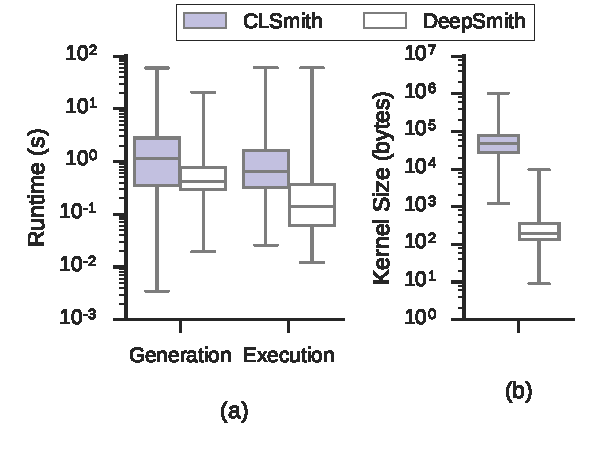
\includegraphics[width=\columnwidth]{build/img/vs-clsmith}%
  \vspace{-1em}
  \caption{%
    Comparison of runtimes (a) and test case sizes (b). DeepSmith test cases are on average evaluated $3.03\times$ faster than CLSmith ($2.45\times$, and $4.46\times$ for generation and execution, respectively), and are two orders of magnitude smaller. Timings do not include the cost of timeouts which would increase the performance gains of DeepSmith by nearly a factor of two.
    % Runtimes, excluding timeouts. .%
%    Total speedup is 3.03x
%    CLgen generation is 2.45x faster than CLSmith
%    CLgen execution is 4.46x faster than CLSmith
%    CLgen reduction is 66.54x faster than CLSmith
  }%
  \label{fig:vs-clsmith} %
\end{figure}

Table~\ref{tab:megatable} shows the results of 48 hours of consecutive testing for all Testbeds. An average of 15k CLSmith and 91k DeepSmith test cases were evaluated on each Testbed, taking an average time per test case of 12.1s and 1.90s respectively. There are three significant factors providing the sixfold increase in testing throughput achieved by DeepSmith over CLSmith: test cases are faster to generate, test cases are less likely to timeout (execute for 60 seconds without termination), and the test cases which do not timeout execute faster.

Figure~\ref{fig:vs-clsmith}a shows the generation and execution times of DeepSmith and CLSmith test cases, excluding timeouts\footnote{If timeouts are included then the performance improvement of DeepSmith is $6.5\times$ with the execution times being $11\times$ faster. However, this number grows as we change the arbitrary timeout threshold, so for fairness to CLSmith we have chosen to exclude it.}. DeepSmith generation time grows linearly with program length, and is on average $2.45\times$ faster than CLSmith. Test case execution is on average $4.46\times$ faster than CLSmith.

The optimization level generally does not affect testing throughput significantly, with the exception of Testbed $7+$. Optimization of large structs is expensive on Testbed $7+$, and CLSmith test cases use global structs extensively. This is a known issue --- in~\cite{Lidbury2015a} the authors omit large-scale testing on this device for this reason. The use of structs in handwritten OpenCL is comparatively rare --- only 7.1\% of kernels on GitHub use them.

% \cc{TODO: Characterisation of OpenCL bug discussion}

\paragraph{Comparison of Test Cases} %
The average CLSmith program is 1189 lines long (excluding headers). CLSmith test cases require reduction in order to expose the underlying bug. An automated approach to OpenCL test case reduction is presented in~\cite{Pflanzer2016}, though it requires on average 100 minutes for each test case using a parallelized implementation (and over 6 hours if this parallelization is not available); the authors also suggest a final manual pass after automated reduction. In contrast, DeepSmith learned to program from humans, and humans do not typically write such large kernel functions. The average DeepSmith kernel is 20 lines long, which is interpretable without reduction, either manual or automatic.

% CLSmith program sizes:
%+--------+-----------+--------+
%| minlen | meanlen   | maxlen |
%+--------+-----------+--------+
%|     56 | 1186.8496 |  11222 |
%+--------+-----------+--------+
% DeepSmith:
%+--------+---------+--------+
%| minlen | meanlen | maxlen |
%+--------+---------+--------+
%|      1 | 20.3163 |    636 |
%+--------+---------+--------+

% TODO: no thread control flow

% TODO: no floats

% TODO: single input

\paragraph{Comparison of Results} %
Both testing systems found anomalous results of all types.
%
% bc column:
% CLSmith generated 3800 silent build crashes. CLgen generated 1023 silent build crashes. Lets ignore these, since we can't be sure of the cause.
% CLSmith triggered 2 distinct compiler assertions. DeepSmith triggered 31.
% CLSmith triggered 0 distinct compiler ``unreachable'' errors. DeepSmith triggered 3.
In 48 hours of testing, CLSmith discovered compile-time crashes (\bc) in 8 of the 20 testbeds, DeepSmith crashed all of them. DeepSmith triggered 31 distinct compiler assertions, CLSmith 2. Both of the assertions triggered by CLSmith were also triggered by CLgen. DeepSmith also triggered 3 distinct \emph{unreachable!} compile-time crashes, CLSmith triggered 0.

The Intel CPU Testbeds ($4\pm$, $5\pm$, $6\pm$, and $7\pm$) would occasionally emit a stack trace upon crashing, identifying the failure point in a specific compiler pass. CLSmith triggered such crashes in 4 distinct passes. DeepSmith triggered crashes in 10 distinct passes, including 3 of the 4 in which CLSmith did. Figure~\ref{lst:intel-passes} provides examples. Many of these crashes are optimization sensitive, and are more likely to occur when optimizations are enabled. CLSmith was able to induce a crash in only one of the Intel testbeds with optimizations disabled. DeepSmith crashed all of the compilers with both optimizations enabled and disabled.

% DeepSmith triggered crashes in ten Intel passes, including three of the four which CLSmith triggered (the one missing one is \emph{Paketize function}).

% CLSmith crash passes:
% Combine Redundant instructions
% Packetize function
% Post-dominance Frontier Construction
% Predicator
%
% DeepSmith crash passes:
% Add SPIR related module scope metadata
% Combine Redundant instructions <- CLSmith triggered this too
% Intel OpenCL Barrier
% LoopWIAnalysis
% Post-dominance frontier construction <- CLSmith triggered this too
% Predicator <- CLSmith triggered this too
% PrepareKernelArgs
% RemoveDuplicateBarrier
% Simplify the CFG
% X86 DAG

\begin{figure}
  \centering
  % Result id: 110876
  \subfloat[\emph{Post-Dominance Frontier Construction} pass.]{%
    \noindent\mbox{\parbox{\columnwidth}{\usebox{\IntelPostDominanceFrontier}}}%
  }\\%
  \subfloat[\emph{Simplify the CFG} pass.]{%
    \noindent\mbox{\parbox{\columnwidth}{\usebox{\SimplifyTheCFGPass}}}%
  }\\%
  % Program id: 31656
  \subfloat[\emph{Predicator} pass.]{%
    \noindent\mbox{\parbox{\columnwidth}{\usebox{\IntelPredicator}}}%
  }\\%
  \subfloat[\emph{Combine redundant instructions} pass.]{%
    \noindent\mbox{\parbox{\columnwidth}{\usebox{\IntelCombineRedundant}}}%
  }\\%
  % Program id: 10596
  \subfloat[\emph{PrepareKernelArgs} pass.]{%
    \noindent\mbox{\parbox{\columnwidth}{\usebox{\IntelPrepareKernelArgs}}}%
  }\\%
  % Program id: 37443
  \subfloat[\emph{Add SPIR related module scope metadata} pass.]{%
    \noindent\mbox{\parbox{\columnwidth}{\usebox{\IntelSPIRMetadata}}}%
  }\\%
  % Program id: 44105
  \subfloat[\emph{Intel OpenCL RemoveDuplicationBarrier} pass.]{%
    \noindent\mbox{\parbox{\columnwidth}{\usebox{\IntelRemoveDupeBarrier}}}%
  }\\%
  \subfloat[\emph{X86 DAG->DAG Instruction Selection} pass.]{%
    \noindent\mbox{\parbox{\columnwidth}{\usebox{\DagPass}}}%
  }\\%
  \caption{Example kernels which crash Intel compiler passes.}%
  \label{lst:intel-passes}
\end{figure}

% bto column:

CLSmith produced many \bto results across 13 Testbeds. Given the large kernel size, it is unclear how many of those are infinite loops or simply a result of slow compilation of large kernels. The average size of CLSmith \bto kernels is 1558 lines. Automated test case reduction --- in which thousands of permutations of a program are executed --- may be prohibitively expensive for test cases with very long runtimes. DeepSmith produced \bto results across 11 Testbeds and with an average kernel size of 9 lines, allowing for rapid identification of the underlying problem.


\begin{figure}
  \centering %
  \subfloat[Assertion \emph{storing/loading pointers only support private array}.]{%
    \noindent\mbox{\parbox{\columnwidth}{\usebox{\BeigPtrAssertion}}}%
    \label{lst:beig-ptr-assertion}
  }\\%
  \subfloat[Assertion \emph{iter != pointerOrigMap.end()}.]{%
    \noindent\mbox{\parbox{\columnwidth}{\usebox{\BeigIterAssertion}}}%
    \label{lst:beig-iter-assertion}
  }\\%
  \caption{Example kernels which trigger compiler assertions which both CLSmith and DeepSmith exposed.}%
  \label{lst:beig-assertions}
\end{figure}

The integrated GPU Testbeds ($3\pm$) frequently failed to compile CLSmith kernels, resulting in over 10k \bc and \bto results.
% 10,318
% SELECT stderr,COUNT(*) FROM CLSmithResults LEFT JOIN CLSmithMetas ON CLSmithResults.id=CLSmithMetas.id WHERE testbed_id=13 AND CLSmithResults.outcome='bc' AND cumtime < 48 * 3600 GROUP BY CLSmithResults.stderr;
Of the build crashes, 68\% failed silently, and the remainder were caused by the same two compiler assertions for which DeepSmith generated 4 line test cases, shown in Figure~\ref{lst:beig-assertions}. DeepSmith also triggered silent build crashes in Testbeds $3\pm$, and a further 8 distinct compiler assertions.

% bf column: CLSmith generated 1 unique build failure (empty declaration). DeepSmith generated 6 unique build failures (including the same empty declaration as CLSmith).
The 4719 \abf results for CLSmith on Testbeds $4\pm$ and $6\pm$ are all a result of compilers rejecting empty declarations, (e.g. \texttt{int;}) which CLSmith occasionally emits. DeepSmith also generated these statements, but with a much lower probability, given that it is an unusual construct (0.6\% of test cases, versus 7.0\% of CLSmith test cases).
% https://github.com/ChrisLidbury/CLSmith/issues/7
Similarly, Testbeds 4--7 reject DeepSmith kernels which omit a type specifier (e.g. \texttt{global* a}), whereas all other Testbeds emit a warning and default to \texttt{int} type.

% c column

% \cc{TODO: CLSmith Testbed $8-$ crashes, Testbed $2-$ crashes}

ComputeAorta (Testbeds $9\pm$) defers kernel compilation so that it can perform optimizations dependent on runtime parameters. This may contribute to the relatively large number of \arc results and few \bc results of Testbeds $9\pm$. Only DeepSmith was able to expose compile-time defects in this compiler.

% CLSmith triggered 2 distinct crashes. DeepSmith triggered 2. Both produced silent crashes where we can't be sure of the cause.

% w column: CLSmith produced 51 distinct wrong-output test cases. Conservatively, let's assume they'll all interesting. DeepSmith produced 69 distinct wrong-output test cases. Conservatively, let's assume that only the bug reports we've submitted are interesting (3).
Over the course of testing, a combined $3.4 \times 10^8$ lines of CLSmith code was evaluated, compared to $3.8 \times 10^6$ lines of DeepSmith code. This provides CLSmith a greater potential to trigger miscompilations. CLSmith generated 33 programs with anomalous wrong-outputs. DeepSmith generated 30.


\subsection{Compiler Stability over Time}%
\label{subsec:clangs}

The Clang front-end to LLVM supports OpenCL, and is commonly used in OpenCL drivers. This in turn causes Clang-related defects to potentially affect multiple compilers, for example the one in Figure~\ref{lst:almost-everything-crash}. To evaluate the impact of Clang, we used debug+assert builds of every LLVM release in the past 24 months and processed 75,000 DeepSmith kernels through the Clang front-end (this includes the lexer, parser, and type checker, but not code generation).

Figure~\ref{fig:clangs} shows that the crash rate of the Clang front-end is, for the most part, steadily decreasing over time. The number of failing compiler crashes decreased tenfold between 3.6.2 and 5.0.0.
%\cc{Does that suggest that DeepSmith is finding bugs which developers are interested in fixing?} \pp{We do find interesting bugs, but the important question is whether we are more likely to find interesting bugs than CLSmith.}
Table~\ref{tab:clangs} shows the 7 distinct assertions triggered during this experiment. Assertion 1 (\emph{Uncorrected typos!}) is raised on all compiler versions --- see Figure~\ref{lst:oclgrind-uncorrected-typos} for an example. The overall rate at which the assertion is triggered has decreased markedly, although there are slight increases between some releases. Notably, the current development trunk has the second lowest crash rate, but is joint first in terms of the number of unique assertions. Assertions 3 (\emph{Addr == 0 || hasTargetSpecificAddressSpace()}) and 4 (\emph{isScalarType()}) were triggered by some kernels in the development trunk but not under any prior release. \factcheck{We have submitted bug reports for each of the three assertions triggered in the development trunk, as well as for two distinct unreachables}.

The results emphasize that compiler validation is a moving target. Every change and feature addition has the potential to introduce regressions or new failure cases. Since LLVM will not release unless their compiler passes their own extensive test suites, this also reinforces the case for compiler fuzzing. We believe our approach provides an effective means for the generation of such fuzzers, at a fraction of the cost of existing techniques.


\subsection{Extensibility of Language Model}

To evaluate the 

Solidity, the programming language of the Ethereum Blockchain. Very young language, little time to develop tooling (yet still very important - money is involved!). Syntax based on JavaScript.

Method: Assembled corpus from scraped solidity files on GitHub. Recursively inlined imported modules. Encoded corpus using combination of tokens and characters (super easy list of tokens were taken from a syntax highlighter). No variable renaming, just code formatting using clangformat. Trained model in the same manner as OpenCL. \cc{TODO: How long did training take?} Simple compile-only test harness. Two testbeds: reference compiler \texttt{solc} with optimizations on or off.

Results from running generator+harness loop for 12 hours. Found a compiler crash caused by missing error handling of language features.
% Unimplemented feature: FixedPointType
% https://github.com/ethereum/solidity/issues/409
%
% /build/solc-GCChSM/solc-0.4.18/libsolidity/codegen/CompilerUtils.cpp(499): Throw in function void dev::solidity::CompilerUtils::convertType(const dev::solidity::Type&, const dev::solidity::Type&, bool, bool, bool)
% Dynamic exception type: boost::exception_detail::clone_impl<dev::solidity::UnimplementedFeatureError>
% std::exception::what: Not yet implemented - FixedPointType.
% [dev::tag_comment*] = Not yet implemented - FixedPointType.
%
Found one case where the compiler silently crashes when optimizations are enabled.
% select * from results
% left join testcases on results.testcase_id=testcases.id
% left join programs on testcases.program_id=programs.id
% left join stderrs on results.stderr_id=stderrs.id
% where programs.generator=1
% and results.id=135558;
%
Triggered one compiler assertion in the emscripten compiled version.
% /usr/local/lib/node_modules/solc/soljson.js:1
% (function (exports, require, module, __filename, __dirname) { var Module;if(!Module)Module=(typeof Module!=="undefined"?Module:null)||{};var moduleOverrides={};for(var key in Module){if(Module.hasOwnProperty(key)){moduleOverrides[key]=Module[key]}}var ENVIRONMENT_IS_WEB=typeof window==="object";var ENVIRONMENT_IS_WORKER=typeof importScripts==="function";var ENVIRONMENT_IS_NODE=typeof process==="object"&&typeof require==="function"&&!ENVIRONMENT_IS_WEB&&!ENVIRONMENT_IS_WORKER;var ENVIRONMENT_IS_SHELL=!ENVIRONMENT_IS_WEB&&!ENVIRONMENT_IS_NODE&&!ENVIRONMENT_IS_WORKER;if(ENVIRONMENT_IS_NODE){if(!Module["print"])Module["print"]=function print(x){process["stdout"].write(x+"\n")};if(!Module["printErr"])Module["printErr"]=function printErr(x){process["stderr"].write(x+"\n")};var nodeFS=require("fs");var nodePath=require("path");Module["read"]=function read(filename,binary){filename=nodePath["normalize"](filename);var ret=nodeFS["readFileSync"](filename);if(!ret&&filenam
% abort() at Error
%     at jsStackTrace (/usr/local/lib/node_modules/solc/soljson.js:1:19718)
%     at stackTrace (/usr/local/lib/node_modules/solc/soljson.js:1:19901)
%     at Object.abort (/usr/local/lib/node_modules/solc/soljson.js:18:10818)
%     at _abort (/usr/local/lib/node_modules/solc/soljson.js:1:828102)
%     at gIa (/usr/local/lib/node_modules/solc/soljson.js:9:380344)
%     at rFa (/usr/local/lib/node_modules/solc/soljson.js:9:305250)
%     at oxa (/usr/local/lib/node_modules/solc/soljson.js:8:845873)
%     at Array._wa (/usr/local/lib/node_modules/solc/soljson.js:8:813044)
%     at Object.GZa [as dynCall_iiiiii] (/usr/local/lib/node_modules/solc/soljson.js:9:725673)
%     at invoke_iiiiii (/usr/local/lib/node_modules/solc/soljson.js:1:863594)
% If this abort() is unexpected, build with -s ASSERTIONS=1 which can give more information.

\cc{Other Notes on Extensibility:} This approach could be combined with symbolic execution to drive more complex structured inputs~\cite{Braione2017}. For dynamic languages, the test process would be the same, only without the separate compilation step and possibility for ``compile-only'' stubs.
